\chapter{Project Design}

In this chapter, we describe the design of the experiment. This chapter will be the
requirements of our pipeline needs to meet also the context it operates in. The two-phase
methodology used for the architecture search and optimizer comparison.


\section{Requirement Analysis}

We have a clear set of requirements for our pipeline. It should have certain outputs and has defined quality.
Set goals and work within a set of limits. This is a computing research project,
Not a software product is. Thus, the requirements are towards reproducibility, numerical accuracy,
and disciplined experimentation.

\subsection{Functional and Nonfunctional Requirements}

The functional requirements describe the actions that the pipeline performs in each phase. Beginning at the pipeline's creation
the reference solution to producing the final comparison report. The nonfunctional requirements determine the quality level. There are two strict requirements – reproducibility and reference accuracy.

\begin{table}[H]
\centering
\caption{Functional Requirements of the Research Pipeline}
\label{tab:fr}
\renewcommand{\arraystretch}{1.2}
\begin{tabular}{|p{1.2cm}|p{12.5cm}|}
\hline
\textbf{ID} & \textbf{Requirement} \\
\hline
FR1 & The system shall be required to generate a high-accuracy numerical reference solution for The Lorenz-1960 ODE system using the fourth-order Runge-Kutta and the SciPy library, evaluated over the interval $t \in [0, 1]$ at $1001$ uniformly spaced points. \\
\hline
FR2 & The system shall partition the reference dataset into training and validation subsets using 80/20 random split with a fixed random seed. \\
\hline
FR3 & The system shall construct feedforward ANN models with systematically varied parameters.
These parameters include depth (1 to 4 hidden layers), width (20, 50, or 100 neurons per layer),
and activation function (tanh, ReLU, sigmoid, GELU, or Swish). \\
\hline
FR4 & The system shall train all Phase 1 models under identical conditions using the Adam optimizer and record convergence behaviour for each run. \\
\hline
FR5 & The system shall conduct a Phase 2 optimizer comparison using the three best Phase 1 architectures.
Each architecture will be trained with Adam, L-BFGS, and SGD with mo momentum.mentum.
momentum. \\
\hline
FR6 & The system shall evaluate each trained model using MSE, MAE, maximum absolute error, training time, and inference time against the RK4 reference. \\
\hline
FR7 & The system shall produce comparison tables, solution trajectory plots, and error curves for every evaluated models. \\
\hline
\end{tabular}
\end{table}

\begin{table}[H]
\centering
\caption{Nonfunctional Requirements of the Research Pipeline}
\label{tab:nfr}
\renewcommand{\arraystretch}{1.2}
\begin{tabular}{|p{1.5cm}|p{12.2cm}|}
\hline
\textbf{ID} & \textbf{Requirement} \\
\hline
NFR1 & All experiments shall be fully reproducible using a single fixed random seed applied to weight initialization and data splitting. \\
\hline
NFR2 & The numerical reference solution shall maintain solver agreement of RMSE below $10^{-10}$ between the custom RK4 implementation and SciPy. \\
\hline
NFR3 & All results, model configurations, and metrics shall be logged systematically so that an independent reader can verify the reported findings. \\
\hline
\end{tabular}
\end{table}

\subsection{Context Diagram}

Figure~\ref{fig:context} shows the research pipeline as one bounded system with two external entities.
The first is a research team. We set up experiments and start them as well as gather the results.
the resulting models and metrics. The second are the academic and research community.
They eat the reported results, repeat the approach and extend the comparisons.
results. Each internal process such as reference generation, final reporting, and so on resides within the
pipeline. There are no other living processes outside the system boundary.


\begin{figure}[H]
\centering
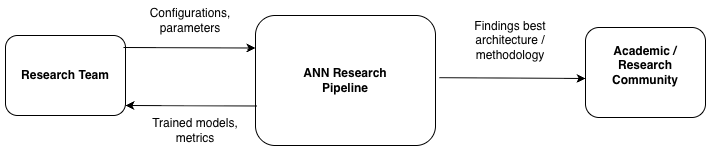
\includegraphics[width=0.85\textwidth]{context_diagram.png}
\caption{Context diagram of the research pipeline.}
\label{fig:context}
\end{figure}

\subsection{Data Flow Diagram Level 1}

Figure~\ref{fig:dfd1} divides the research pipeline into a series of five steps. Process P1 generates
Plot the reference trajectory with both the RK4- and SciPy-solvers. P2 makes it preprocess the trajectory
It is done through the 80/20 split and z-score normalization of the output targets.
P3 trains the ANN models, initially over the complete Phase 1 grid, and subsequently over the Phase 2
optimizer comparison. P4 test each of the trained models with the reference solution
using the metrics from FR6. P5 compares the results, selects the best architecture and Creates the final report.

\begin{figure}[ht]
\centering
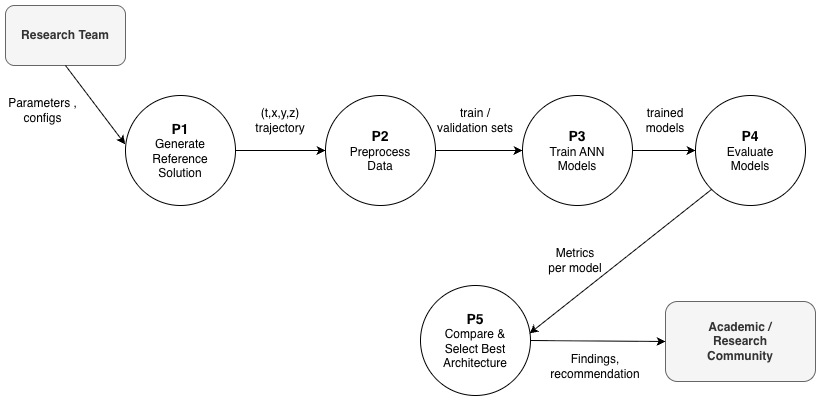
\includegraphics[width=0.95\textwidth]{dfd_level1.png}
\caption{Data Flow Diagram (Level 1) showing the five internal processes of the research pipeline.}
\label{fig:dfd1}
\end{figure}

\subsection{UI Design}

This project has no user interface. We run everything from Python scripts and Jupyter notebooks. Results are stored as figures, tables, and serialized model files. UI design does not apply here.

\section{Detailed Methodology and Design}

The methodology is divided into two phases. Here is the logic.

\begin{itemize}
    \item \textbf{Phase 1 -- Architecture Search (60 runs):} We choose the depth: 1--4 hidden layers, width: 20, 50, 100 neurons, and activation functions: tanh, ReLU, Sigmoid, GELU and Swish. Also we choose the optimizer fixed at Adam. This will show us which architectural choices matter most.
    \item \textbf{Phase 2 -- Optimizer Comparison (9 runs):} We take the three best architectures from Phase 1. Then fine-tune each one with the following three algorithms: Adam, L-BFGS, SGD with momentum. All other factors remain unchanged.All other factors remain constant. This indicates the percentage of optimization that the optimizer will use to
contributes on top of the architecture.

\end{itemize}

This separation allows that the two comparisons are not confused. If any
Improvements in Phase 2 do not result from optimizing the network, but from a change in the network structure.


\subsection{Reference Solution Generation}

We calculate the reference solution from the Lorenz-1960 system with $k=2$, $l=1$, initial conditions $x(0)=0.5$, $y(0)=0.75$, $z(0)=1$, and time interval $t \in [0, 1]$, as defined in Chapter~2. Two independent solvers are used to ensure that reference numbers are accurate. The first is a custom-made fourth-order Runge-Kutta integrator with step size $h=10^{-3}$ . Evaluated at a common grid of points $1001$ points. The second one is the solve ivp of SciPy  routine using DOP853 with $\text{rtol}=10^{-10}$ and $\text{atol}=10^{-12}$ which is sampled on the same grid. We need agreement between both solvers at RMSE below $10^{-10}$ and then we use
The RK4 trajectory was adopted as the reference trajectory for training and evaluation of all the ANNs. This dual solver are make sure to check and catch the unintentional mistakes in either implementation. Also it provides us a reliable reference and the rest of the study will be based on this.

\subsection{Dataset Preparation}

The reference trajectory provides us with $1001$ ,$(t, x(t), y(t), z(t))$. That is our training set. Our training set is 80\% training (around $800$ points) and our validation set is 20\% validation (about $201$ points) and we report our results on the validation set. The data is split randomly into two halves, with seed $42$. It comes as a surprise to us all but we do the split once before training any model. All configurations of the ANN use the same training points, validation points, and validation error.The same training points, the same validation points, and the same validation error are used in every ANN configuration.
and in the same order. 
We then normalize each of the three target variables by using the training-set,
the mean and standard deviation. Given $x$ , $y$ and $z$ , this $z$ score normalization puts $x$ , $y$ and $z$ on a comparable scale, to ensure that the loss function is not being swamped by the variable with the largest range of variation range. The key to this is that all errors are reported after unnormalisation. The published metrics stay in the original physical units of the system.


\subsection{Model Family and Architecture (Phase 1)}

Each candidate ANN is a simple feedforward network.  Accepts scalar time $t$ as an argument, it is used for predicting the three dimentional state vector $(x(t), y(t), z(t))$. The hidden structure varies with The number of hidden layers, the number of neurons in each hidden layer, activation function. We explore these values in Phase 1 as listed in Table~\ref{tab:phase1grid}. 

The Cartesian product of these axes results in $4 \times 3 \times 5 = 60$ distinct architectures. We
Optimize each one separately with the same optimization parameters. The output layer is
always linear with three units. We do not include any skip connections, normalization layers, and
no regularization. This is a simple design on purpose. It helps hold the comparison to one's mind. From our research question about the three architectural axes, the following questions were developed.


\begin{table}[H]
\centering
\caption{Phase 1 Architecture Search Grid}
\label{tab:phase1grid}
\renewcommand{\arraystretch}{1.2}
\begin{tabular}{|l|l|}
\hline
\textbf{Axis} & \textbf{Values} \\
\hline
Depth (hidden layers) & 1, 2, 3, 4 \\
\hline
Width (neurons per layer) & 20, 50, 100 \\
\hline
Activation function & tanh, ReLU, sigmoid, GELU, Swish \\
\hline
Total configurations & $4 \times 3 \times 5 = 60$ \\
\hline
\end{tabular}
\end{table}

\subsection{Optimizer Comparison (Phase 2)}

Phase 2 takes the three architectures with the lowest combined validation MSE from Phase 1 and retrains each one with two additional optimizers: L-BFGS and SGD with momentum. Everything else stays the same as Phase 1. We reuse the Adam result from Phase 1 as the third comparison point. That gives us $3 \times 3 = 9$ Phase 2 runs.

Why these optimizers? L-BFGS is a strong baseline for smooth, low-dimensional regression problems. Researchers commonly cite it as effective for ANN-based ODE solvers. SGD with momentum serves as a classical reference. This phase isolates the optimizer's effect from the network architecture's effect. This separation would not be achievable if optimizer selection were included in the Phase 1 search grid.

\subsection{Loss Function and Training Protocol}

The training loss is the mean squared error between the normalized predicted state and the normalized reference state, computed jointly over all three output components. We add no initial-condition penalty and no physics-based residual. This is consistent with the plain-ANN scope from Chapter~2 and avoids the loss-balancing problem that plagues physics-informed approaches.

Here are the training settings:

\begin{itemize}
    \item Phase 1 uses Adam with learning rate $10^{-3}$ and default momentum parameters.
    \item Each model trains for at most $10{,}000$ epochs.
    \item Early stopping monitors validation loss with a patience of $500$ epochs and restores the best-validation weights when training ends.
    \item We use full-batch gradient descent. The training set is small enough that full-batch is appropriate, and it removes minibatch noise as a confounding variable across configurations.
    \item We set the PyTorch random seed to $42$ before constructing each model, so weight initialization is reproducible too.
\end{itemize}


\subsection{Evaluation Metrics}
The results of each model trained are tested and compared with the RK4 reference result.
using 5 metrics. Table ~\ref{tab:metrics}  lists them. MSE is the major indicator as it corresponds to This training goal and allows them to compare all the configurations directly. The absolute
error and the maximum absolute error are the reported per state variable. They provide a
more comprehensible representation of the best and worst scenarios deviations. Training
time relates to the amount of the cost to train a particular architecture. Inference time
represents the cost of prediction of the complete trajectory when it is trained. Together,
These five are the indicators that will help us in our search of the accuracy/cost trade-off we're looking for our research question.

\begin{table}[H]
\centering
\caption{Evaluation Metrics Used for Each Trained Model}
\label{tab:metrics}
\renewcommand{\arraystretch}{1.2}
\begin{tabular}{|l|p{9.5cm}|}
\hline
\textbf{Metric} & \textbf{Purpose} \\
\hline
MSE (per variable and combined) & Primary loss. Consistent comparison across all $69$ runs \\
\hline
MAE (per variable) & Interpretable error magnitude in original physical units \\
\hline
Maximum absolute error & Worst-case deviation along the trajectory \\
\hline
Training time (seconds) & Computational cost of fitting a given architecture \\
\hline
Inference time (seconds) & Cost of predicting the full $1001$-point trajectory after training \\
\hline
\end{tabular}
\end{table}

\subsection{Alternative Solutions Considered}

We looked at several alternatives before settling on the plain feedforward ANN with a pure MSE loss. Here is what we rejected and why.

A PINN would re-use the hyperparameter and add a residue term to the loss.Balancing problem described in Chapter 2. It also would make it difficult to distinguish between our work The current PinnDE research and the ongoing PinnDE study. So we dropped it.

The same reason was rejected for a DeepONet operator-learning approach. PinnDE
A DeepONet is already tested by already on the same equation. The reproduction of that design would not address the architecture-selection gap that we found.


We explored the possibility of a Neural ODE formulation as it is a different paradigm. However, Neural ODEs do not parameterize the solution function, they parameterize the derivative. That does not give an answer to our research question

Lastly, we considered fusing the architecture search and an optimizer selection as a single process. We did not accept this as there would be more experiments in total. And mix the two effects we wish to separate from each other. The two phase design while still maintaining a clean attribution of the, adopted has the number of runs at 69 observed differences.

\section{Project Plan}

The project plan is a research design that is designed to be carried out over 42 weeks in the following way: FYDP-I, FYDP-II, and FYDP-III. The schedule groups the work into research and writing, baseline and data preparation, implementation, analysis and validation, presentation and The timeline is based on the sequence of submission milestones, according to the scope of the problem. Results verification, report, framing and numerical baseline validation to ANN experiments Completing and defence preparation. Each of the three phases are 14 weeks long, with the last one being a deliberate review. 2 weeks will be dedicated to each phase of the defense preparation and final presentation. The task placement is provided in Figure ~\ref{fig:fydp_gantt} and Table ~\ref{tab:gantt_task_ids} shows the placement across the three 14-week trimesters. Specifies the names in the chart.


\begin{figure}[H]
\centering
\caption{42-week FYDP Gantt chart using task IDs.}
\label{fig:fydp_gantt}
\resizebox{\textwidth}{!}{%
\begin{ganttchart}[
    hgrid,
    vgrid,
    x unit=0.28cm,
    y unit chart=0.31cm,
    bar height=0.42,
    group height=0.24,
    milestone height=0.34,
    group label font=\bfseries\tiny,
    bar label font=\bfseries\tiny,
    milestone label font=\bfseries\tiny,
    title label font=\tiny\bfseries,
    title height=0.7,
    group/.append style={fill=black!45},
    milestone/.append style={fill=red!70},
    progress label text={}
]{1}{42}
\gantttitle{FYDP-I}{14}
\gantttitle{FYDP-II}{14}
\gantttitle{FYDP-III}{14} \\
\gantttitle{1}{1}
\gantttitle{}{5}
\gantttitle{7}{1}
\gantttitle{}{5}
\gantttitle{14}{2}
\gantttitle{}{5}
\gantttitle{21}{2}
\gantttitle{}{5}
\gantttitle{28}{2}
\gantttitle{}{5}
\gantttitle{35}{2}
\gantttitle{}{5}
\gantttitle{42}{2} \\
\ganttgroup{FYDP-I}{1}{14} \\
\ganttbar[bar/.append style={fill=blue!55}]{T01}{1}{2} \\
\ganttbar[bar/.append style={fill=blue!55}]{T02}{3}{6} \\
\ganttbar[bar/.append style={fill=blue!55}]{T03}{7}{10} \\
\ganttbar[bar/.append style={fill=teal!60}]{T04}{8}{12} \\
\ganttbar[bar/.append style={fill=orange!70}]{T05}{11}{12} \\
\ganttbar[bar/.append style={fill=orange!70}]{T17}{13}{14} \\
\ganttmilestone{M01}{14} \\
\ganttgroup{FYDP-II}{15}{28} \\
\ganttbar[bar/.append style={fill=teal!60}]{T06}{15}{16} \\
\ganttbar[bar/.append style={fill=green!55}]{T07}{15}{20} \\
\ganttbar[bar/.append style={fill=green!55}]{T08}{19}{23} \\
\ganttbar[bar/.append style={fill=green!55}]{T09}{23}{25} \\
\ganttbar[bar/.append style={fill=purple!55}]{T10}{20}{26} \\
\ganttbar[bar/.append style={fill=orange!70}]{T11}{24}{26} \\
\ganttbar[bar/.append style={fill=orange!70}]{T18}{27}{28} \\
\ganttmilestone{M02}{28} \\
\ganttgroup{FYDP-III}{29}{42} \\
\ganttbar[bar/.append style={fill=purple!55}]{T12}{29}{32} \\
\ganttbar[bar/.append style={fill=purple!55}]{T13}{31}{34} \\
\ganttbar[bar/.append style={fill=blue!55}]{T14}{33}{36} \\
\ganttbar[bar/.append style={fill=blue!55}]{T15}{35}{39} \\
\ganttbar[bar/.append style={fill=orange!70}]{T16}{38}{40} \\
\ganttbar[bar/.append style={fill=orange!70}]{T19}{41}{42} \\
\ganttmilestone{M03}{42}
\end{ganttchart}%
}

\vspace{0.5em}
\scriptsize
\begin{tabular}{lll}
\textcolor{blue!70}{\rule{1em}{0.8em}} Research and writing &
\textcolor{teal!70}{\rule{1em}{0.8em}} Baseline and data &
\textcolor{green!70}{\rule{1em}{0.8em}} Implementation \\
\textcolor{purple!70}{\rule{1em}{0.8em}} Analysis and validation &
\textcolor{orange!80}{\rule{1em}{0.8em}} Presentation &
\textcolor{red!75}{\rule{1em}{0.8em}} Milestone
\end{tabular}
\end{figure}

\begin{table}[H]
\centering
\caption{Task and Milestone IDs Used in the Gantt Chart}
\label{tab:gantt_task_ids}
\scriptsize
\renewcommand{\arraystretch}{1.08}
\begin{tabularx}{\textwidth}{@{}p{0.7cm}>{\raggedright\arraybackslash}X>{\centering\arraybackslash}p{1.0cm}p{0.7cm}>{\raggedright\arraybackslash}X>{\centering\arraybackslash}p{1.0cm}@{}}
\toprule
\textbf{ID} & \textbf{Task or Milestone} & \textbf{Weeks} &
\textbf{ID} & \textbf{Task or Milestone} & \textbf{Weeks} \\
\midrule
T01 & Problem framing and objectives & 1--2 & T10 & Metrics, logging, and visualizations & 20--26 \\
T02 & Literature review and gap analysis & 3--6 & T11 & Chapter 4 draft and presentation & 24--26 \\
T03 & Requirements and standards mapping & 7--10 & T18 & Defense preparation and final presentation & 27--28 \\
T04 & Baseline validation and dataset specification & 8--12 & M02 & FYDP-II submission milestone & 28 \\
T05 & Interim report and presentation & 11--12 & T12 & Result verification and reproducibility review & 29--32 \\
T17 & Defense preparation and final presentation & 13--14 & T13 & Comparative analysis and final figures & 31--34 \\
M01 & FYDP-I submission milestone & 14 & T14 & Standards, constraints, and impact analysis & 33--36 \\
T06 & Canonical dataset generation & 15--16 & T15 & Final report revision and conclusion & 35--39 \\
T07 & ANN training pipeline implementation & 15--20 & T16 & Final presentation and defense preparation & 38--40 \\
T08 & Phase 1 architecture search & 19--23 & T19 & Defense preparation and final presentation & 41--42 \\
T09 & Phase 2 optimizer comparison & 23--25 & M03 & Final submission and defense & 42 \\
\bottomrule
\end{tabularx}
\end{table}

\section{Task Allocation}
There are 5 members in our team. We divided up tasks by skill area and also mapped all of the members' contributions to FYDP-I, FYDP-II and FYDP-III. This prevents treating the
write chapters without regard to the rest of the book. All members are involved in the same research pipeline consisting of a variety of planning to final defense with different primary ownership.


\begin{table}[H]
\centering
\caption{Task Allocation Across Team Members and FYDP Segments}
\label{tab:tasks}
\scriptsize
\renewcommand{\arraystretch}{1.2}
\begin{tabularx}{\textwidth}{|p{2.4cm}|>{\raggedright\arraybackslash}X|>{\raggedright\arraybackslash}X|>{\raggedright\arraybackslash}X|}
\hline
\textbf{Member} & \textbf{FYDP-I Responsibilities} & \textbf{FYDP-II Responsibilities} & \textbf{FYDP-III Responsibilities} \\
\hline
Ikramul Hasan Moral & Lead numerical baseline validation; verify the Lorenz-1960 equation setup; define data-generation requirements. & Implement preprocessing, model definitions, training loop, and experiment runner for the $69$ planned runs. & Recheck reproducibility, archive scripts and results, and support technical defense of the implementation. \\
\hline
Md. Abu Bakar & Support requirements analysis and metric selection; review literature related to evaluation criteria. & Build the evaluation pipeline; compute MSE, MAE, maximum error, training time, and inference time. & Consolidate final tables; verify result consistency against the requirements; support analysis discussion. \\
\hline
Samiur Rahman Omlan & Prepare methodology diagrams and initial experimental workflow documentation. & Produce convergence plots, solution trajectory plots, and architecture-comparison figures. & Finalize visual evidence for Chapter~4 and presentation slides; support result interpretation. \\
\hline
Fariha Islam & Lead literature review, gap analysis, citation tracking, and Chapters~1--2 drafting. & Maintain citation consistency while implementation details are added to Chapter~4. & Revise the final report for academic tone, citation coverage, and defense-readiness. \\
\hline
Md. Touhidul Islam & Compile Chapter~3 planning material, task allocation, and interim-report structure. & Coordinate weekly documentation, report updates, and experiment-log summaries. & Compile the final report, Chapter~5 constraints, Chapter~6 conclusion, and final presentation narrative. \\
\hline
\end{tabularx}
\end{table}

All members participate in supervisor meetings, progress journals, internal result reviews, and FYDP presentations. Shared review is necessary because an error in the solver, dataset, model configuration, or interpretation would affect the whole research conclusion.

\section{Summary}

 Chapter 1 into a conceptual framework.The research question from Chapter 1 and literature gap from Chapter 1 was transformed into a conceptual framework in this chapter. Chapter 2 into a concrete experimental design. Functional requirements tell you what the pipeline must yield and the non-functional requirements tell you the quality the pipeline must achieve. The context
The pipeline is put in its research environment by diagram and Level 1 data flow diagram.
A two-phase comparative study methodology is used. A 60-configuration phase 1 run is executed. Search over depth, width and activation function for architecture. Phase 2 is a 9 configuration optimizer comparison of the three best architectures. This means 69 controlled experiments altogether. We calculate reference data and check it on two different solvers.
We keep training, loss and evaluation settings fixed for all the runs so that they are observed . The differences are attributable to variables studied. The project plan assigns the work to the three segments of FYDP (each 14 weeks). There is a two-week period for defense preparation and the final presentation at the end of each phase. The items have been captured as tasks T17, T18 and T19 in the revised 42-week schedule. The task allocation Delegates team members to implementation, analysis and writing. In the next chapter, the implementation of this design and the experimental results from it are reported 69 runs.
